\documentclass{article}

\usepackage{caption}
\usepackage{subcaption}
\usepackage{amsmath}

\usepackage{arxiv}

\usepackage[utf8]{inputenc} % allow utf-8 input
\usepackage[T1]{fontenc}    % use 8-bit T1 fonts
\usepackage{hyperref}       % hyperlinks
\usepackage{url}            % simple URL typesetting
\usepackage{booktabs}       % professional-quality tables
\usepackage{amsfonts}       % blackboard math symbols
\usepackage{nicefrac}       % compact symbols for 1/2, etc.
\usepackage{microtype}      % microtypography
\usepackage{lipsum}
\usepackage{graphicx}

\usepackage{algorithm2e}


\usepackage{authblk}

\usepackage[backend=biber]{biblatex}
\addbibresource{refs.bib}

% allow long URLs in the bibliography to break across lines
\setcounter{biburlnumpenalty}{9000}
\setcounter{biburlucpenalty}{9000}
\setcounter{biburllcpenalty}{9000}

\graphicspath{ {./fig/} }

\usepackage{tikz}
\usetikzlibrary{arrows.meta, bending, positioning}

\newcommand{\map}{\mathop{\bigoplus}\limits}
\newcommand{\txtop}[1]{\mathop{\mathtt{#1}}\limits}

\newcommand{\expr}{\txtop{expression}}

\newcommand{\fn}{\txtop{function}}
\newcommand{\linear}{\txtop{linear}}
\newcommand{\relu}{\txtop{ReLU}}
\newcommand{\topk}{\txtop{TopK}}
\newcommand{\sigmoid}{\txtop{sigmoid}}
\newcommand{\tanhl}{\txtop{tanh}}
\newcommand{\softmax}{\txtop{softmax}}
\newcommand{\argmin}{\txtop{argmin}}
\newcommand{\argmax}{\txtop{argmax}}
\newcommand{\einsum}{\txtop{einsum}}
\newcommand{\colsum}{\txtop{colsum}}

\newcommand{\encoder}{\txtop{encoder}}
\newcommand{\decoder}{\txtop{decoder}}
\newcommand{\classifier}{\txtop{classifier}}
\newcommand{\partitioner}{\txtop{dict}}

\newcommand{\bilinearblock}{\txtop{BilinearBlock}}
\newcommand{\dictblock}{\txtop{DictBlock}}
\newcommand{\dictenc}{\txtop{DictEnc}}
\newcommand{\ontologizer}{\txtop{Ontologizer}}

\SetKwProg{Fn}{Function}{}{end}
\SetKwProg{Dat}{Data}{}{end}

\SetKwInOut{Hyper}{Hyperparameters}

\SetKwFunction{softmax}{softmax}
\SetKwFunction{MSE}{MSE}
\SetKwFunction{L1}{L1}
\SetKwFunction{transpose}{transpose}
\SetKwFunction{matmul}{matmul}
\SetKwFunction{dist}{dist}
\SetKwFunction{eucl}{euclidean}
\SetKwFunction{cossim}{cossim}
\SetKwFunction{sindiff}{sindiff}
\SetKwFunction{pca}{pca}
\SetKwFunction{knn}{knn}

\SetKwFunction{sample}{sample}
\SetKwFunction{loss}{loss}
\SetKwFunction{train}{train}

\SetKwFunction{Type}{Type}
\SetKwFunction{List}{List}
\SetKwFunction{Arch}{Arch}
\SetKwFunction{Params}{Params}
\SetKwFunction{Model}{Model}

\SetKwFunction{Linear}{Linear}
\SetKwFunction{Bilinear}{Bilinear}
\SetKwFunction{NLinear}{NLinear}
\SetKwFunction{NLinearBlock}{NLinearBlock}
\SetKwFunction{DictBlock}{DictBlock}
\SetKwFunction{DictEnc}{DictEnc}
\SetKwFunction{Ontologizer}{Ontologizer}
\SetKwFunction{SAE}{SAE}


\date{\today}

\title{A proposal for mixture-of-experts-based interpretability}

\author[1]{Keira Wiechecki}
\affil[1]{Wakaru, \texttt{kaw504@nyu.edu}}

\begin{document}
\maketitle

\begin{abstract}
  
  %Adapting this method to nontrivial models will be involved, but I expect it to represent a substantial advance in interpretability.  
\end{abstract}

worked:
pointless vector space
subspaces of cluster
graph theory

didn't:
dimension reduction 
algebraic 
topology

\section{Assumptions}

methods/assumptions"
- steering is inherent to the training objective  (interpretability steering isomorphism) (the dictionary vectors must also be high quality steering vectors)
- assumption that weights are themselves interpretable
- clustering rather than decomposition (actually the clustering thing is counterintuitive if you don't bring leiden)
- imposing categorical structure on feature (ontology vs typology. also relates to a related work.)
- cheap interpretability "forward pass"
- straightforward composition of concepts (concepts must be composable to be useful)
- (nonstandard) dictionary learning is all you need 
- the dictionary forms a basis for the representantion rather than a target
- representations are not themselves quantized (the learned dictionary serves as a basis for the representation rather than a discrete codebook. quantization comes from sharpening of classifications over said basis)
- interpreting a well trained model is the same as interpreting the data/training tasks.

\subsection{Pivotal assumptions}
Some version of the linear representation hypothesis
Latent space is ``natural''

\subsection{Concerns}

\paragraph{Timelines could be too short}
We'll just have to go faster.

\paragraph{Contrastive classifiers might not be expressive enough}

\paragraph{Steering could push it too far off manifold}
%(diffusive steering? activation steering? still gives good data to test steering methods) (can we RL a model on high activations vs. low activations for given classification? does it converge faster than normal contrastive pairs/arbitrary PCA vector?)
This is an open problem in mechinterp. Diffusion steering is one candidate to address it\cite{wagenmaker2025}.
If we can't solve the problem it still gives good data to test steering methods. e.g. can we RL a model for high/low scores on a classification and have it converge faster than paired steering or PCA vectors?

\paragraph{Representations could be too soft/dense/high entropy}
%(highly correlated across all feature-based interp i.e. SAEs, transcoders, J-space)
This is highly correlated across all feature-based interp (SAEs, transcoders, J-space). Dividing representations across orthogonal categorical subspaces makes it possible to interpret the conceptual basis vectors even if the representations are dense mixtures.

\paragraph{Ontofeatures could be too polysemantic}
%(theoretical inductive bias, as long as they have decent explanatory power we can do eigendecomposition; we have more directions to increase parameters)
Orthogonality \& categorical constraints give a theoretical inductive bias to monosemanticity.
As long as they have decent explanatory power we can do eigendecomposition; polysemanticity decreases with parameter count and we have more directions to increase parameters (in addition to increasing width we can increase head size or stack more layers)

\paragraph{Interpreting ontofeatures could be otherwise intractable}
%(implies SLT is false)
This would imply the universality hypothesis is false and is highly correlated with intractability of other interpretability agendas. Submodules could be interpretable even if features aren't.

\paragraph{Training could be intractable}
%(sparsity trades against sample/compute efficiency; we have less need for sparsity constraint)
Sparsity trades against sample/compute efficiency; preliminary experiments suggest we have less need for a sparsity constraint.

\paragraph{Too many hyperparameters/too hyperparameter dependent}
%(becomes less of an issue with scaling; qualitatively seems to just converge slower)
This generally becomes less of an issue with scaling; preliminary experiments show most changes to hyperparameters just change the rate of convergence.

\paragraph{Doesn't converge in the limit}
%(collapse propagates down layers) (underparameterised, really bad optimizer, bad initialization, bad loss function)
\paragraph{not orthogonal in the limit}

\paragraph{might not generalize out of distribution}

\paragraph{inference too expensive}

\paragraph{autointerp doesn't work on parameters/eigenfeatures}

\section{Theory of change}
Conditional on my underlying model of ontology being true, 
I'm ~80\% confident that the techniques I propose will be a substantial interpretability advance.
Moreover, I believe the proposed research agenda to have a high counterfactual impact.
Because the theoretical basis consists of nonobvious applications of obscure techniques from 
niche fields of bioinformatics, I'm 50\% confident that similar research would not be done in the 
next 2 years otherwise.

\subsection{What I expect a solution to look like}
I believe (~50\%) that mechinterp offers the best path to a robust alignment solution despite
\href{https://www.lesswrong.com/posts/tEPHGZAb63dfq2v8n/how-useful-is-mechanistic-interpretability}{criticisms}.
This is based on 
\begin{enumerate}
    \item \textbf{decomposability} Mechinterp allows alignment to be broken into manageable subproblems.
    \item \textbf{parallelizability} Decomposable subproblems can be worked on independently.
    \item \textbf{robustness} Mechinterp offers direct causal explanations of model behavior.
\end{enumerate}
The most straightforward mechinterp alignment solutions are
\begin{enumerate}
    \item \href{https://www.alignment.org/blog/arcs-first-technical-report-eliciting-latent-knowledge/}{eliciting latent knowledge (ELK)} 
    Directly inferring a model's ontology.
    \label{it:elk}
    \item \href{https://www.alignment.org/blog/mechanistic-anomaly-detection-and-elk/}{mechanistic anomaly detection (MAD)} 
    Detecting when a model has ``unusual'' thoughts.
    \label{it:mad}
\end{enumerate}
Both of these can be considered 
\href{https://arbital.greaterwrong.com/p/ontology_identification/}{ontology identification}
subproblems. 
MAD requires mapping between the model's activations and the model's ontology.
ELK requires mapping between the model's ontology and human ontology.
These are hard but not intractable problems.
Recently, \href{https://devinterp.com/}{developmental interpretability} 
(devinterp) techniques have enabled identification of ``developmental stages'' 
corresponding to learning specific tasks.
\cite{hoogland2024developmental}.
This is strong evidence that learning consists primarily of the network
grokking\cite{nanda2023progress} discrete concepts.
While these results are promising for MAD, 
locating these emergent capabilities in the model's activations remains an open problem.

\subsection{My macro-scale strategy}
%I see the fundamental problems for alleviating this threat as
Broadly, my goals are to
\begin{enumerate}
  \item formalize the notion of a model's latent concept space
  \item distill a model's latent concept space
  \item enforce decomposability of latent concept space
  \item enforce robustness of existing concepts as the dimensionality of the latent concept space increases
\end{enumerate}

A prerequisite for all of these is the ability to express a 
\href{https://plato.stanford.edu/entries/ontological-commitment/}{metaontology}
which can identify latent concepts in activation space.

The dominant paradigm in mechanistic interpretability is to treat a model as a finite state
machine

\section{Background}
Mechanistic interpretability currently can do supervised steering well or unsupervised steering poorly. 
This has prompted the Google Deep Mind interpretability team to pivot to a pragmatic steering 
agenda\cite{gdmprogress2025}. 
Compared to unsupervised interpretability, supervised steering is highly robust.
However it can only distinguish what the experimenter is looking for
and does not account for the actual computations performed by a model\cite{makelov2023}.
The dominant unsupervised paradigm is the sparse autoencoder (SAE).
A model's hidden state is approximated as a finite state machine consisting of discrete features.
The initial implementation used a $\relu$ activation and sparsity loss\cite{bricken2023},
though more recent implemetations have used a $\topk$ activation function without a sparsity loss\cite{gao2024}.

\subsection{Common problems with SAEs}
The motivation is to decompile a model to a finite state machine (FSM). 
The limitation is that such an FSM only as interpretable as an enumeration of all possible states.

\subsubsection{Features are not composable}
A persistent problem with SAEs is feature absorption\cite{chanin2025}.
Instead of representing an input as a composition of monosemantic features,
an SAE will often instead use a single separate feature.
This is a problem for interpretability, as we would like features to generalize.
One attempt to address this problem is Matryoshka SAEs\cite{bussmann2025},
which use multiple layers to build a hierarchical coarse-to-fine representation.

\subsubsection{Features are not causal}
Sparsity trades off against reconstruction fidelity.
Using features for steering often results in inconsistent, context-sensitive behavior\cite{duan2026}.

\subsubsection{Features are not closed-form}
A major concern is how well an interpretability technique generalizes out-of-distribution.
Ideally we would like to infer behavior by looking solely at model weights,
which can be achieved with bilinear MLPs\cite{pearce2025}.

\subsubsection{Forward passes are expensive}
Efficiency is also a problem. Although the sparsity constraint means that only a handful of 
features are active for a given input, the entire feature space needs to be computed\cite{} for each sample.
Mixture-of-experts (MoE) SAE variants reduce compute costs by dividing feature space between smaller
submodules. Examples include Switch SAEs\cite{mudide2025} and Tree SAEs\cite{cao2026}.

Less explored is the effect of the structure imposed by the MoEfied architecture on the interpretability of feature space.
A common approach to scalably interpreting features is using an LLM to predict activations from examples\cite{paulo2025}.
With an unstructured feature space, it quickly becomes intractable to interpret all 
permutations of features this way. It is however possible to instead apply this technique to 
expert routings.
The MLPs of a transformer can themselves be converted to an MoE architecture\cite{zhang2022}.
Language models seem to organize contrastive concepts into orthogonal simplices\cite{park2025}.
This is suggestive of MoEfication revealing latent contrastive steering vectors.
Imposing an orthogonality constraint has been shown to significantly reduce feature
absorption\cite{korznikov2025}.

This assumes that
\begin{itemize}
	\item Some version of the linear representation hypothesis is true
	\item Latent space is in some way ``natural''
\end{itemize}

\section{Methods}

\subsection{Architecture}
We propose a novel method which encodes samples as classifications mapped to contrastive vectors.
This directly constrains a model's representations.
Moreover, classifications can natively be used for steering.

The model (Figure~\ref{fig:onto-stack}) is a stack of $l$ dictionary layers
writing into a shared residual accumulator, decoded by a single linear map.
Each layer (Figure~\ref{fig:dictenc}) splits into $h$ independent heads; a head
classifies its input over $k$ dictionary entries and emits the corresponding
convex combination of them. The softmax is what carries the contrastive
structure: within a head the entries are mutually exclusive alternatives rather
than independently firing features (Figure~\ref{fig:head-simplex}), so a
classification is a well-defined object to intervene on.

% Ontologizer architecture figures.
%
% Requires only what paper.tex already loads:
%   tikz + \usetikzlibrary{arrows.meta, positioning}, amsmath,
%   caption, subcaption.
%
% Values annotated on the diagrams are the live SONAR configuration
% (sonar.py): d = 1024, e_dec = 2048, k = 32, h = 32, l = 5, n = 2
% (bilinear), forward = "resid", deepsup = True, resid_norm = True,
% resid_const = True, encoded = False, scaled = False.

% =====================================================================
% (1) the layer stack
% =====================================================================
\begin{figure}[tp]
\centering
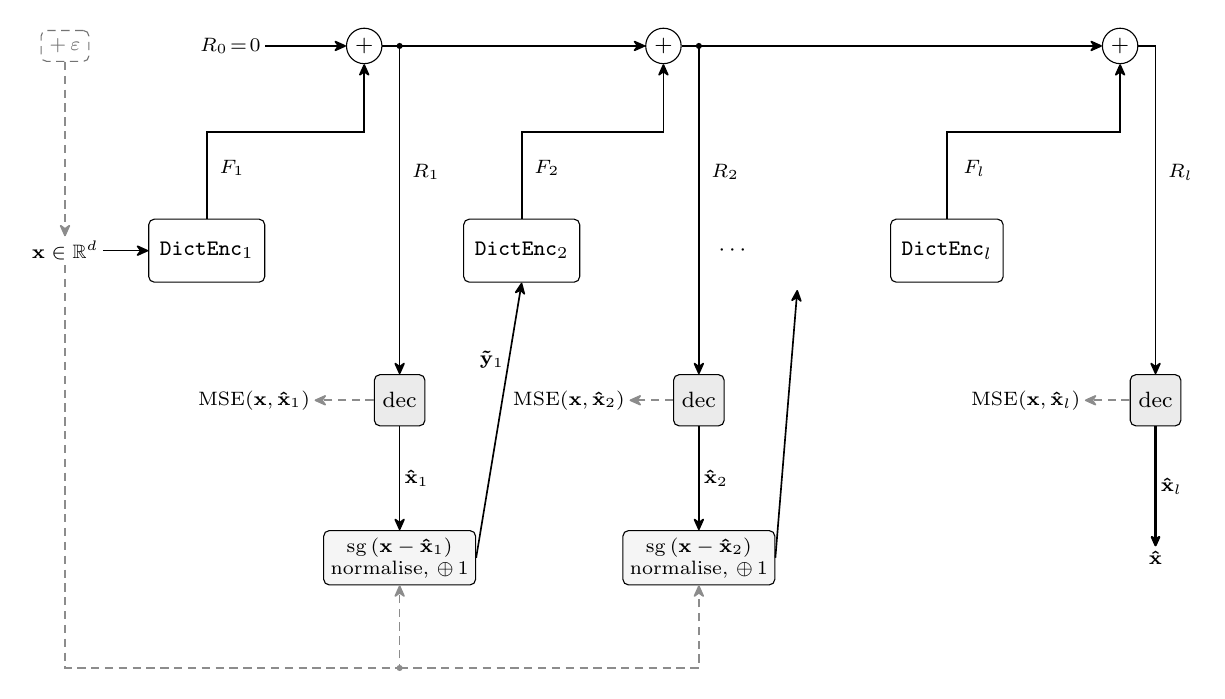
\begin{tikzpicture}[
    font=\footnotesize,
    >={Stealth[round,length=1.8mm,width=1.6mm]},
    blk/.style={draw, rounded corners=2pt, align=center,
                minimum height=8mm, inner xsep=4pt},
    hook/.style={draw, rounded corners=2pt, densely dashed, align=center,
                 inner sep=3pt, font=\scriptsize, black!55},
    dec/.style={draw, rounded corners=2pt, fill=black!8,
                minimum height=6.5mm, inner xsep=3pt},
    cond/.style={draw, rounded corners=2pt, fill=black!4, align=center,
                 inner sep=2.5pt, font=\scriptsize},
    add/.style={draw, circle, minimum size=4.5mm, inner sep=0pt},
    lab/.style={inner sep=1.5pt, font=\scriptsize},
    sig/.style={->, semithick},
    aux/.style={->, densely dashed, semithick, black!45},
  ]

  %% ---- layer row --------------------------------------------------
  \node[lab] (x)  at (-1.5,0) {$\mathbf{x}\in\mathbb{R}^{d}$};
  \node[blk] (D0) at ( 0.3,0) {$\mathtt{DictEnc}_1$};
  \node[blk] (D1) at ( 4.3,0) {$\mathtt{DictEnc}_2$};
  \node      (Dd) at ( 7.0,0) {$\cdots$};
  \node[blk] (DL) at ( 9.7,0) {$\mathtt{DictEnc}_{l}$};

  \draw[sig] (x) -- (D0);

  \node[hook] (noise) at (-1.5,2.6) {$+\,\varepsilon$};
  \draw[aux] (noise) -- (x);

  %% ---- residual accumulator (top rail, y = 2.6) --------------------
  \node[add] (A0) at ( 2.3,2.6) {$+$};
  \node[add] (A1) at ( 6.1,2.6) {$+$};
  \node[add] (AL) at (11.9,2.6) {$+$};

  \node[lab] (R0) at (0.6,2.6) {$R_0\!=\!0$};
  \draw[sig]      (R0) -- (A0);
  \draw[sig]      (A0) -- (A1);
  \draw[sig]      (A1) -- (AL);
  \draw[semithick] (AL) -- (12.35,2.6);

  %\node[lab] at (8.9,3.05) {$R\in\mathbb{R}^{e}$: residual accumulator};

  %% ---- per-layer contributions F_i (enter from below) --------------
  \draw[sig] (D0.north) -- ++(0,1.1) -| (A0.south);
  \draw[sig] (D1.north) -- ++(0,1.1) -| (A1.south);
  \draw[sig] (DL.north) -- ++(0,1.1) -| (AL.south);
  \node[lab] at (0.62,1.05) {$F_1$};
  \node[lab] at (4.62,1.05) {$F_2$};
  \node[lab] at (10.05,1.05) {$F_{l}$};

  %% ---- shared decoder, one decode per prefix -----------------------
  \node[dec] (Y1) at ( 2.75,-1.9) {$\mathrm{dec}$};
  \node[dec] (Y2) at ( 6.55,-1.9) {$\mathrm{dec}$};
  \node[dec] (YL) at (12.35,-1.9) {$\mathrm{dec}$};

  \draw[sig] ( 2.75,2.6) -- (Y1.north);
  \draw[sig] ( 6.55,2.6) -- (Y2.north);
  \draw[sig] (12.35,2.6) -- (YL.north);
  \fill ( 2.75,2.6) circle (1.1pt);
  \fill ( 6.55,2.6) circle (1.1pt);

  \node[lab,anchor=west] at ( 2.85,1.0) {$R_1$};
  \node[lab,anchor=west] at ( 6.65,1.0) {$R_2$};
  \node[lab,anchor=west] at (12.45,1.0) {$R_l$};

  %% ---- deep supervision --------------------------------------------
  \node[lab] (L1) at ( 0.9,-1.9) {$\mathrm{MSE}(\mathbf{x},\mathbf{\hat{x}}_1)$};
  \node[lab] (L2) at ( 4.9,-1.9) {$\mathrm{MSE}(\mathbf{x},\mathbf{\hat{x}}_2)$};
  \node[lab] (LL) at (10.7,-1.9) {$\mathrm{MSE}(\mathbf{x},\mathbf{\hat{x}}_l)$};
  \draw[aux] (Y1.west) -- (L1);
  \draw[aux] (Y2.west) -- (L2);
  \draw[aux] (YL.west) -- (LL);

  %% ---- residual forwarding ------------------------------------------
  \node[cond] (C1) at (2.75,-3.9)
  {$\mathrm{sg}\,(\mathbf{x}-\mathbf{\hat{x}}_1)$\\ normalise, $\oplus\,1$};
  \node[cond] (C2) at (6.55,-3.9)
  {$\mathrm{sg}\,(\mathbf{x}-\mathbf{\hat{x}}_2)$\\ normalise, $\oplus\,1$};
  \draw[sig] (Y1) -- node[right,lab]{$\mathbf{\hat{x}}_1$} (C1);
  \draw[sig] (Y2) -- node[right,lab]{$\mathbf{\hat{x}}_2$} (C2);

  \draw[sig] (C1.east) -- node[left,lab,pos=0.72]{$\mathbf{\tilde{y}}_1$} (D1.south);
  \draw[sig] (C2.east) -- (7.8,-0.5);

  %% ---- model output --------------------------------------------------
  \node[lab] (out) at (12.35,-3.9) {$\mathbf{\hat{x}}$};
  \draw[sig,thick] (YL) -- node[right,lab]{$\mathbf{\hat{x}}_l$} (out);

  %% ---- x broadcast to every conditioning step -------------------------
  \draw[aux] (x.south) -- (-1.5,-5.3) -- (2.75,-5.3) -- (C1.south);
  \draw[aux] (2.75,-5.3) -- (6.55,-5.3) -- (C2.south);
  \fill[black!45] (2.75,-5.3) circle (1.1pt);

\end{tikzpicture}


\caption[\texttt{Ontologizer} architecture]{\textbf{\texttt{Ontologizer} architecture.}
	An \texttt{Ontologizer} consists of $l$ stacked \texttt{DictEnc} layers.
	Each returns a feature vector $F_i\in\mathbb{R}^{e}$,
	which is written to a residual accumulator $R$.
	For each layer $i$, $R_i = \mathrm{sg}(R_{i-1}) + F_i$.
	The stop gradient function $\mathrm{sg}$ prevents communication between layers.
	$\mathrm{dec}$ is a linear decoder with shape $\mathbb{R}^{d \times e}$.
	It uses deep supervision to obtain a coarse-to-fine representation where
	the component encoded by previous layers is inaccessible to later layers.
	At each layer $i$, $\mathbf{\hat{x}}_i = \mathrm{dec}(R_i)$.
	The same decoder is shared by all layers.
	The component explained by a layer is given by
	$\mathbf{y}_i = \mathbf{x} - \mathbf{\hat{x}}_i$.
	The input to layer $i+1$ is given by
	$\mathbf{\tilde{y}}_i
	  = \mathbf{y}_i / \mathrm{L2}(\mathbf{y}_i) \oplus [1]$
	where $\mathrm{L2}$ is the unit norm. This prevents exploding gradients from repeated
	application of bilinear layers, as each scales its input by $\lVert\cdot\rVert^{2}$.
	A constant coordinate $[1]$ is appended, giving a dimension of $d+1$.
	This prevents the sign information of $\mathbf{y}_i$ from being lost
	by the bilinear transformation.
	Effectively, it adds a bias to an otherwise unbiased linear form
	while preserving eigendecomposition.

	$\mathrm{MSE}(\mathbf{x},\mathrm{dec}(R_i))$ is computed separately for each layer.
}
\label{fig:onto-stack}
\end{figure}

% =====================================================================
% (2) inside one DictEnc, and the per-head geometry
% =====================================================================
\begin{figure}[tp]
\centering

\begin{subfigure}{\textwidth}
\centering
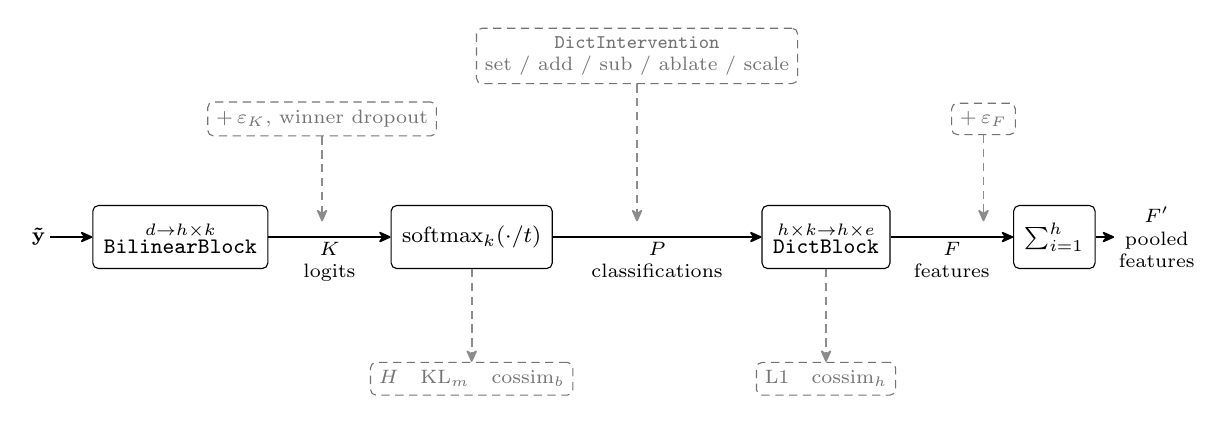
\begin{tikzpicture}[
    font=\footnotesize,
    >={Stealth[round,length=1.8mm,width=1.6mm]},
    blk/.style={draw, rounded corners=2pt, align=center,
                minimum height=8mm, inner xsep=4pt},
    hook/.style={draw, rounded corners=2pt, densely dashed, align=center,
                 inner sep=3pt, font=\scriptsize, black!55},
    lab/.style={inner sep=1.5pt, font=\scriptsize, align=center},
    sig/.style={->, semithick, align=center},
    aux/.style={->, densely dashed, semithick, black!45},
  ]

  %% ---- main chain ----------------------------------------------------
  \node[lab] (E)  at (-0.6,0) {$\mathbf{\tilde{y}}$};
  \node[blk] (CL) at ( 1.2,0) {$\bilinearblock^{d \to h \times k}$};
  \node[blk] (SM) at ( 4.9,0) {$\mathrm{softmax}_k(\cdot/t)$};
  \node[blk] (DB) at ( 9.4,0) {$\dictblock^{h \times k \to h \times e}$};
  \node[blk] (SU) at (12.3,0) {$\sum^{h}_{i=1}$};
  \node[lab] (F)  at (13.6,0) {$F'$\\ pooled\\ features};

  \draw[sig] (E)  -- (CL);
  \draw[sig] (CL) -- node[below,lab]{$K$\\ logits}   (SM);
  \draw[sig] (SM) -- node[below,lab]{$P$\\ classifications}   (DB);
  \draw[sig] (DB) -- node[below,lab]{$F$\\ features} (SU);
  \draw[sig] (SU) -- (F);

  %% ---- training-time hooks and the intervention interface (above) ----
  \node[hook] (nk) at (3.0,1.5) {$+\,\varepsilon_K$,\ winner dropout};
  \node[hook] (iv) at (7.0,2.3) {\texttt{DictIntervention}\\
                                 set / add / sub / ablate / scale};
  \node[hook] (nf) at (11.4,1.5) {$+\,\varepsilon_F$};
  \draw[aux] (nk) -- (3.0,0.20);
  \draw[aux] (iv) -- (7.0,0.20);
  \draw[aux] (nf) -- (11.4,0.20);

  %% ---- where each regulariser attaches (below) -----------------------
  \node[hook] (lp) at (4.9,-1.8)
    {$H$\quad $\mathrm{KL}_m$\quad $\mathrm{cossim}_b$};
  \node[hook] (lf) at (9.4,-1.8)
    {$\mathrm{L1}$\quad $\mathrm{cossim}_h$};
  \draw[aux] (SM.south) -- (lp);
  \draw[aux] (DB.south) -- (lf);

\end{tikzpicture}


\caption[\texttt{DictEnc} architecture]{\textbf{\texttt{DictEnc} architecture.}
	Dashed lines above indicate perturbations to the data,
	including noising and causal interventions.
	Dashed lines below indicate statistics used as tuneable auxiliary loss functions.
	Each \texttt{DictEnc} consists of a multihead bilinear classifier
	($\bilinearblock$) with weights
	$[\mathsf{W}, \mathsf{V}] \in \mathbb{R}^{2 \times h \times k \times d}$
	and a multihead linear dictionary ($\dictblock$)
	with weights $\mathsf{D} \in \mathbb{R}^{h \times e \times k}$.
	It accepts a vector $\mathbf{x} \in \mathbb{R}^{d}$,
	which may be a residual from a previous layer.
	A $\bilinearblock$ accepts inputs $\mathbf{x} \in \mathbb{R}^d$.
	It returns logits $K \in \mathbb{R}^{h \times k}$ given by
	$K = \left(\sum^{d}_{j=1}W_{\cdot,\cdot,j}x_j\right)
	     \odot \left(\sum^{d}_{j=1}V_{\cdot,\cdot,j}x_j\right)$.
	An optional noise term $\varepsilon_K$ may be added.
	Winner dropout sets $\mathrm{argmax}_k(K_{h,\cdot})$ to $-\infty$
	with probability $p_{\mathrm{drop}}$.

	Soft labels $P$ are given by $\mathrm{softmax}_{k}(K/T)$
	where $T$ is a temperature hyperparameter. Over the course of training
	it is annealed from $1.0$ to $0.03$, giving progressively sharper classifications.
	The architecture provides methods for causal interventions on labels.
	From $P$ we collect per-sample entropy $H$,
	between-sample similarity $\mathrm{cossim}_b$,
	and batch mean entropy $\mathrm{KL}_m$.
	In practice $H$ is not needed, as including a
	$\mathrm{cossim}_b$ loss also minimizes $H$.
	$\mathrm{KL}_m$ serves to anchor the batch mean of each label vector
	$\mathbf{p}_{i,\cdot}$ to a uniform distribution.
	This results in a uniform $\mathbf{p}_{i,\cdot}$ code corresponding
	to a maximally generic feature vector.

	A $\dictblock$ accepts labels 
	$P \in \mathbb{R}^{h \times k}$
	and returns features $F \in \mathbb{R}^{h \times e}$ given by
	$F = \sum^{k}_{j=1}\lvert D_{\cdot,\cdot,j}\rvert \, P_{\cdot,j}$.
	Because $\lvert D_{\cdot,\cdot,j}\rvert$ is an absolute value
	and $P_{hj} \in [0,1]$, features are strictly additive.
	From $F$ we collect sparsity penalty $\mathrm{L1}$
	and between-head similarity $\mathrm{cossim}_h$.
	Both $\mathrm{L1}$ and $\mathrm{cossim}_h$ tend to decrease with only
	$\mathrm{MSE}$ loss, but incorporating them into the loss speeds up convergence.
	$\mathrm{cossim}_h$ is of particular interest because it measures
	the extent to which heads encode nonoverlapping geometries.

	We add noise $\varepsilon_F$ to $F$, then sum over the head dimension to obtain
	pooled features $F' \in \mathbb{R}^{e}$, which are added to $R$.
}
\label{fig:dictenc}
\end{subfigure}

\vspace{7mm}

\begin{subfigure}{\textwidth}
\centering
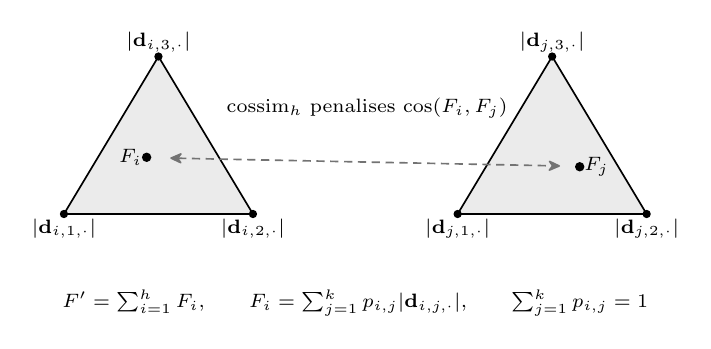
\begin{tikzpicture}[
    font=\footnotesize,
    >={Stealth[round,length=1.8mm,width=1.6mm]},
    lab/.style={inner sep=1.5pt, font=\scriptsize},
  ]
  %% ---- head i --------------------------------------------------------
  \fill[black!8]   (0,0) -- (2.4,0) -- (1.2,2.0) -- cycle;
  \draw[semithick] (0,0) -- (2.4,0) -- (1.2,2.0) -- cycle;
  \fill (0,0)     circle (1.5pt) node[below,lab]{$\lvert \mathbf{d}_{i,1,\cdot}\rvert$};
  \fill (2.4,0)   circle (1.5pt) node[below,lab]{$\lvert \mathbf{d}_{i,2,\cdot}\rvert$};
  \fill (1.2,2.0) circle (1.5pt) node[above,lab]{$\lvert \mathbf{d}_{i,3,\cdot}\rvert$};
  \fill (1.05,0.72) circle (1.7pt) node[left,lab]{$F_i$};

  %% ---- head j -------------------------------------------------------
  \fill[black!8]   (5.0,0) -- (7.4,0) -- (6.2,2.0) -- cycle;
  \draw[semithick] (5.0,0) -- (7.4,0) -- (6.2,2.0) -- cycle;
  \fill (5.0,0)   circle (1.5pt) node[below,lab]{$\lvert \mathbf{d}_{j,1,\cdot}\rvert$};
  \fill (7.4,0)   circle (1.5pt) node[below,lab]{$\lvert \mathbf{d}_{j,2,\cdot}\rvert$};
  \fill (6.2,2.0) circle (1.5pt) node[above,lab]{$\lvert \mathbf{d}_{j,3,\cdot}\rvert$};
  \fill (6.55,0.60) circle (1.7pt) node[right,lab]{$F_{j}$};

  \draw[<->, densely dashed, semithick, black!55] (1.35,0.71) -- (6.30,0.61);
  \node[lab] at (3.85,1.35)
    {$\mathrm{cossim}_h$ penalises $\cos(F_i,F_{j})$};

  \node[lab, anchor=north, align=center] at (3.7,-0.9)
  {$F'=\sum^h_{i=1} F_i$,\qquad
  $F_i=\sum^k_{j=1} p_{i,j}\lvert \mathbf{d}_{i,j,\cdot}\rvert$,\qquad $\sum^k_{j=1} p_{i,j}=1$};
\end{tikzpicture}


\caption[Per-head geometry]{\texttt{DictBlock} \textbf{head geometry} for $h=2$; $k=3$.
	The output space of a head $i$ forms a simplex with the columns of the matrix
	$D_{i,\cdot,\cdot}$ as the vertices. 
	The column vectors $\mathbf{d}_{i,j,\cdot}$ form the spanning set of the
	feature space. Any $F_i$ must be a linear combination of the columns of 
	$D_{i,\cdot,\cdot}$.
	As $F$ becomes sparser, these vectors become more approximately
	orthogonal, allowing them to be treated as a basis.
	The label code $P$ correspond to soft assignments to mutually contrastive
	categories rather than independently firing features.
	Because elements of $P$, $p_ij \in [0,1]$, 
	outputs must be within the convex hull of $D_{i,\cdot,\cdot}$.
	Because $\lvert D\rvert\geq0$ and $P\geq0$, $F\geq0$
	Therefore $\cos(F_i, F_j) \in [0,1]$.
	This means that minimizing $\mathrm{cossim}_h(F)$ 
	pushes the simplices to be disjoint.

  The code is the sum of one such point per
  head. Since $\lvert D\rvert\geq0$, every $F_h$ lies in the non-negative
  orthant and $\cos(F_h,F_{h'})\in[0,1]$, so driving $\mathrm{cossim}_h$ to
  zero demands \emph{disjoint support} between heads --- strictly stronger
  than orthogonality of signed vectors, and the sense in which the
  architecture is built to seek an orthogonal decomposition.}
\label{fig:head-simplex}
\end{subfigure}

\caption{\textbf{One dictionary layer, and the geometry it imposes.}}
\label{fig:dictenc-full}
\end{figure}


\subsection{Training}

\subsubsection{Embedding model}
We embed texts using SONAR\cite{sonar}, a multimodal and language-agnostic sentence embedding 
model. SONAR embeddings have several desirable properties:
\begin{itemize}
	\item They correspond to entire texts rather than tokens.
	\item They are bidirectional.
	\item Language is encoded independently of text.
\end{itemize}
This allows us to validate steering fidelity against a ground truth.

\subsubsection{Loss function}

\subsection{Evaluation}

\section{Preliminary results}

\subsection{Reconstruction quality}

\subsection{Orthogonality}

\subsection{Categorical structure}

\subsection{Automated interpretability}

\subsection{Steering fidelity}

have an underexplored method we believe allows high quality unsupervised steering.
existing attempts to route activations to expert SAEs has focused on routing similar things to the same expert, but actually to do contrastive learning you want to train on things on opposite ends of a shared axis. we don't just want to find similar features, we want to find contrastive vectors in featurespace that correspond to what a model considers a natural category.

\section{Future work}

\subsection{Change in interpretability over training}

\subsection{Transcoder adaptation}

\subsection{HSIC bottleneck}

freyavoice: 
what we're doing glosses broadly as "let humans understand AI". the alternative is get AI to understand humans better.
but you dummies! if you make the AI smarter this is going to lead to subtler and subtler issues with larger and larger effects!

jadevoice:
we're not just letting humans understand AI. because an LLM reflects humanity from the training data, high quality conceptual interpretability provides machine comprehensible mathematical representations of *every concept that humanity cares about*. yes, we're working on interp for the usual corrigibility reasons, but we're also solving one of the most challenging parts of outer alignment - feature representation!

Ideally we would like mechanistic interpretability to provide guarantees about
the computational process used by a model. We would like features to be
1. causal
2. composable
3. closed

However most existing techniques, such as sparse autoencoders (SAEs),
produce features that can perform arbitrarily badly on these desiderata.
Feature splitting breaks compositionality. 
They can't usually be statically analyzed (though bilinear SAE variants can be).
Sparsity trades off against reconstruction fidelity, limiting the extent to which 
features can be used for steering.

Arguably the simplest interpretability technique is a linear probe,
and the simplest control technique is a steering vector.
They are remarkably robust compared to unsupervised techniques such as SAEs,
but require labeled contrastive datasets.
We propose a MoEfication technique based on decomposing a model into a set of 
contrastive classifiers. Each classification corresponds to a representative vector.
Inputs are encoded as a series of classifier outputs, and reconstructed 
from a weighted average of the representative vectors.
This has several advantages over SAEs:
1. It effectively gives steering for free.
2. Outputs are bounded.
3. The representative vectors can be statically interpreted.
4. Feature space is structured.

\subsection{Background}
Bilinear MLPs
Feature Absorption
SONAR
Large Concept Models
Matryoshka SAEs
Switch SAEs
Tree SAE
MoEfication
SAEBench
AxBench
autointerp



\printbibliography

%\input{sections/appendix.tex}

\end{document}
